\documentclass[11pt]{article}    
    \addtolength{\topmargin}{-3cm}
    \addtolength{\textheight}{3cm}
\usepackage{graphicx}
\usepackage[section]{placeins}
\usepackage{geometry}
\usepackage{color,soul}
\usepackage{pdfpages}
\usepackage[noae]{Sweave}



\title{Revised Alert Messages Application}
\author{Peter Higgins, PhD}
\date{November 7, 2021}

\begin{document}
\maketitle




\section{Introduction}

This work is a revision of previous versions that implements changes requested by the project specialist, Elizabeth Waagen, AAVSO, including:

\begin{enumerate}

    \item Restructure star table in html alert message to format RA and DEC into single string with units for them included in header but not in each record. Format is hh mm ss for RA, and dd mm ss for DEC with leading 0 if abs of either less that 10 (so 3 degrees is shown as 03)
    
    \item Automate upload of included table or graphic upon entry of this file in both new submittals and edited submittals.
    
    \item Change input of included graphic to file search control which allows user to select this file from the file manager. 
    
    \item Add AAVSO's forum page as clickable link in alert message html document. 
    
    \item Verify save of feedback so it is shown in edit form.    


In addition to the requested changes above, other changes were made including;

	\begin{enumerate}
	\item Table showing lists of alert messages revised.
	\item Restriction limiting generation of alert messages (HTML) to only those that have been 'approved' has been removed so staff can edit them as a draft document and save the draft separately. 
	\item Submit and edit submit forms improved. 
	\item Action buttons on Submit and edit Submit moved to top of form.
	\end {enumerate}
	\end {enumerate}

\section{Log in as staff member}
Logging in as a staff member directs the user to the page shown in Figure 1 which lists all alert message records currently i the database regardless of submitter. 

\begin{figure}[htp]
\centering
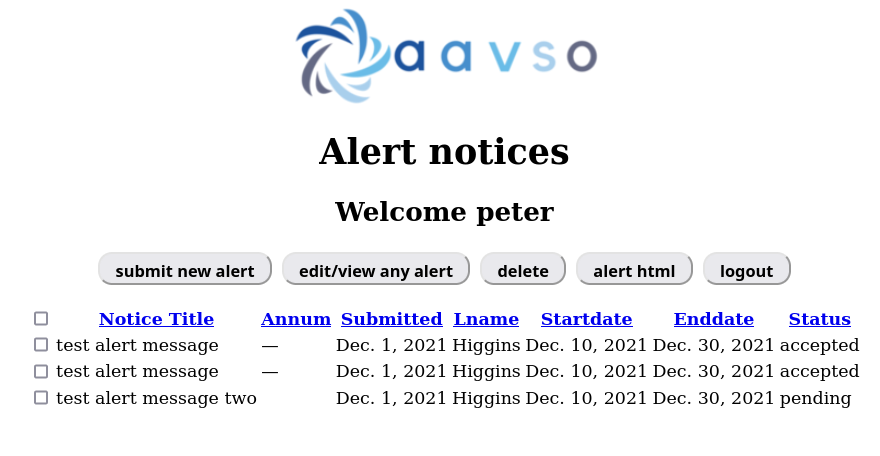
\includegraphics[scale=1.00]{staffmain.png}
\caption{staff login main screen}
\label{staff 1}
\end{figure}

The user actions associated with the buttons are:
\begin{figure}[htp]
\centering
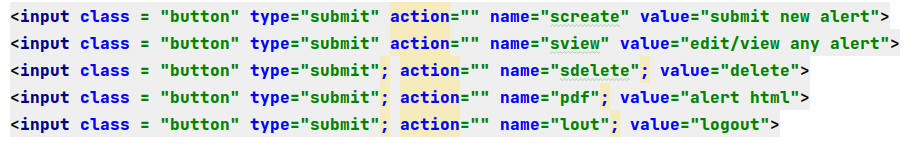
\includegraphics[scale=1.00]{staffmain2.png}
\caption{staff login main button actions}
\label{staff 2}
\end{figure}
\subsection{staff create submittal}
Clicking on the button "submit new alert" directs to this code in views.py:
\begin{figure}[htp]
\centering
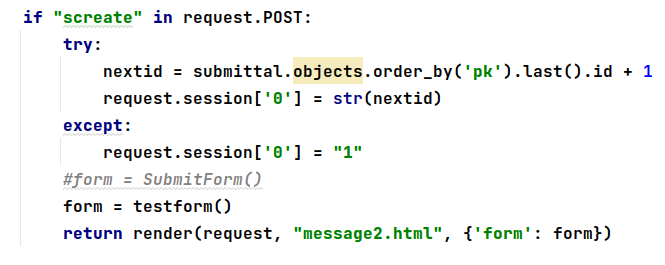
\includegraphics[scale=1.00]{staffmain3.png}
\caption{code for staff create new message}
\label{staff 3}
\end{figure}
This code does 3 things:
\begin{itemize}
\item establishes the id to use for the new record as 1 more than the last.
\item saves the id as session variable
\item initiates a sunmit form which is message2.html. (in this case a test form for easy testing)
\end {itemize}
The called screen (return render) identified by message2 is shown as:
\begin{figure}[htp]
\centering
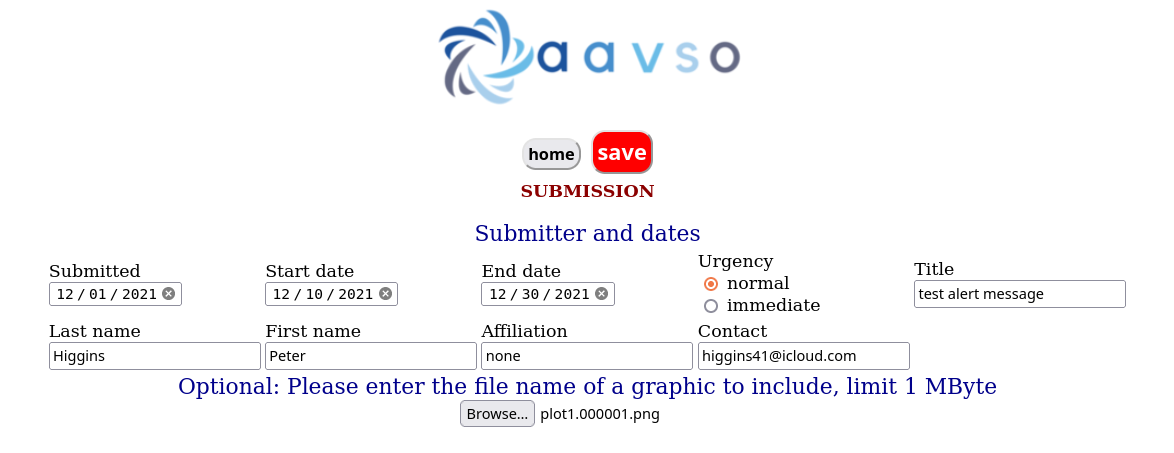
\includegraphics[scale=1.00]{staffmain4.png}
\caption{form for staff create}
\label{staff 4}
\end{figure}
Here it is seen that:
\begin{itemize}
\item Action buttons moved to top, save button in red
\item Button to get included graphic changed to FileField for file manager selection.
\end{itemize}
When this form is complete and saved, its botton half is given in Figure 5:
\begin{figure}[htp]
\centering
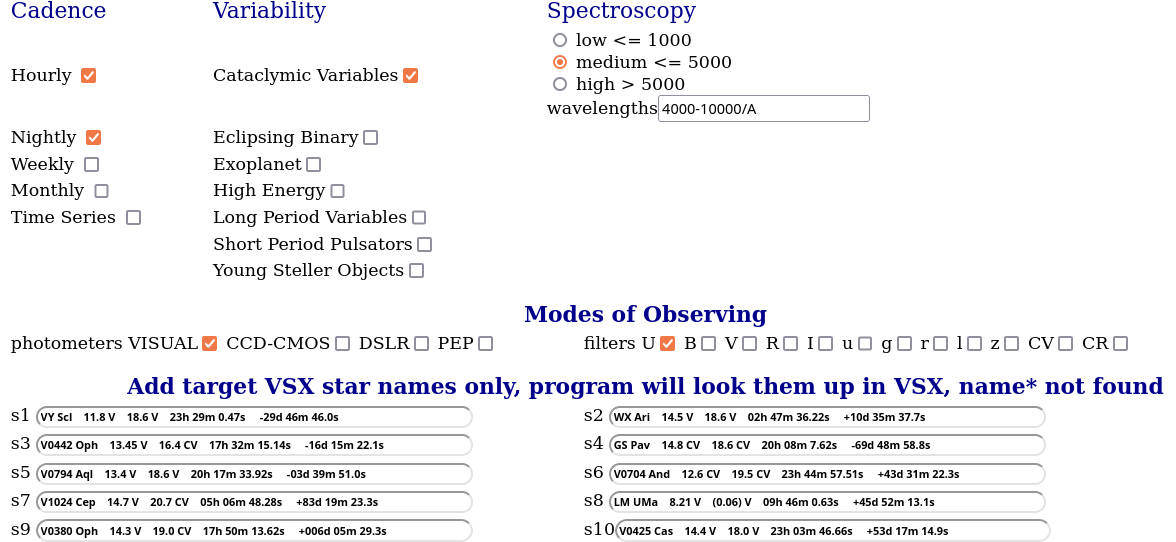
\includegraphics[scale=1.00]{staffmain5.png}
\caption{bottom of staff create form}
\label{staff 5}
\end{figure}
\begin{itemize}
\item Close examination of figure 5 shows that leading zeros are added when needed as well as "+-" on Declination. 
\item Examination of the database confirms that the include file 'plot1.0000001.png and the star data have been stored in the database as confirmed by Figures 6 and 7:
\end{itemize}
\begin{figure}[htp]
\centering
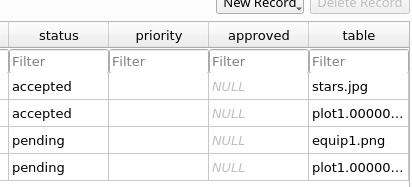
\includegraphics[scale=1.00]{staffmain7.png}
\caption{bottom of staff create form}
\label{staff 6}
\end{figure}
 as well as the stars. 
\begin{figure}[htp]
\centering
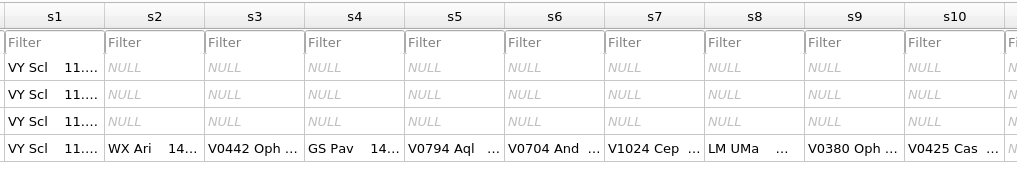
\includegraphics[scale=1.00]{staffmain8.png}
\caption{bottom of staff create form}
\label{staff 7}
\end{figure}


\subsection{staff edit submittal}
Clicking on the button "edit/view any alert" directs to this code in views.py as shown in figure 8:
\begin{figure}[htp]
\centering
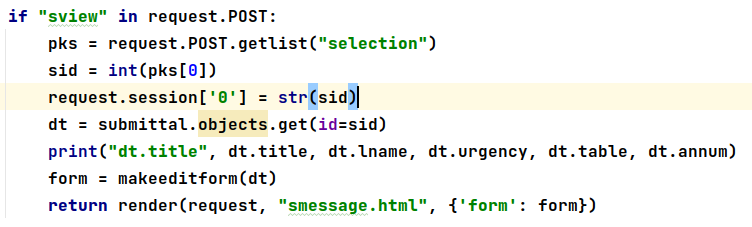
\includegraphics[scale=1.00]{staffmain10.png}
\caption{staff edit submittal code}
\label{staff 10}
\end{figure}
\begin{itemize}
\item The edit code captures the submitall record checked
\item It creates a queryset dictionary for the record which is printed as a diagnostic
\item It initializes an edit form which is displayed using template "smessage.html"
\item "smessage.html" is rendered as shown in Figure 9.
\end{itemize}
\begin{figure}[htp]
\centering
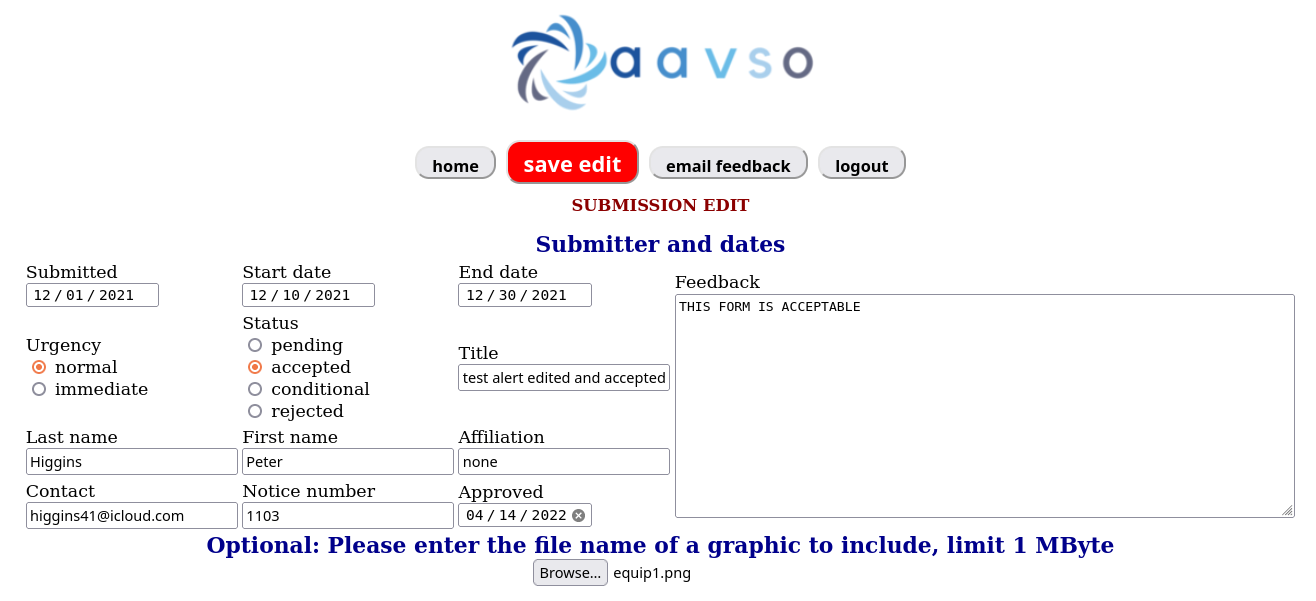
\includegraphics[scale=0.6]{staffedit1.png}
\caption{staff edit form}
\label{staff 14}
\end{figure}
Figure 9 shows that:
\begin{itemize}
\item Action buttons have been moved to the edit form's top with the save button colored red. 
\item A large input control has been added on the edit form for feedback to the alert message poster that can be emailed to that person's contact address.
\item Saving the edit correctly loads new values in the database, and uploads the included graphic (IT IS EMPHASIZED THAT THE USER MUST CHOSE AN INCLUDED GRAPHIC FILE EVEN IF IT IS THE SAME AS ON THE ORIGINAL RECORD.) 
\item A FileField input control is used for file selection.
\item This staff edit form permits changing the message status such as "approved".
\end{itemize}
\subsection{staff edit save edited form}

\subsection{staff edit email feedback}
\begin{figure}[htp]
\centering

\includegraphics[scale=0.4]{staffemail.png}
\caption{staff edit feedback email}
\label{staff email}
\end{figure}
The code for the email is shown here:
\begin{figure}[htp]
\centering
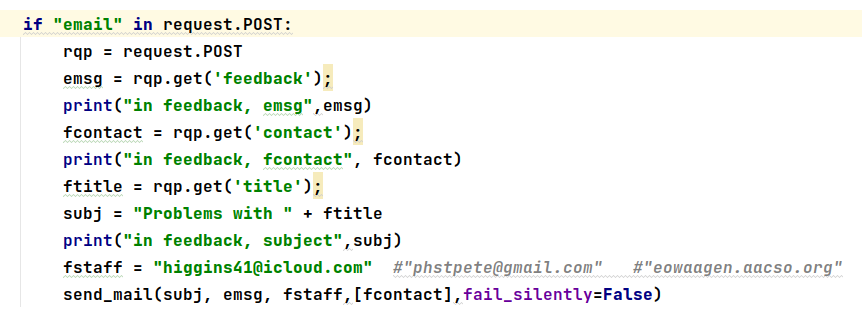
\includegraphics[scale=0.4]{staffemailcode.png}
\caption{staff email code}
\label{staffemail code}
\end{figure}

\end {document}
